\documentclass[12pt,fleqn]{article}
\usepackage{xiiiemc}
\usepackage{natbib}
\usepackage{fancyhdr}
\usepackage{fancyvrb}
\usepackage{color}
\usepackage{wallpaper} 
\usepackage{titlesec}   %% Define space between paragraph e section
\usepackage{float} 	%% Use to fix Figure or Table: ex: \begin{table}[H]
\usepackage[usenames,dvipsnames]{xcolor}
\usepackage{hyperref} 	%% Use to fix Figure or Table: ex: \begin{table}[H]
\hypersetup{
	%pagebackref=true,
	pdfcreator={LaTeX with abnTeX2},
	pdfkeywords={abnt}{latex}{abntex}{USPSC}{trabalho acadêmico}, 
	colorlinks=true,       		% false: boxed links; true: colored links
	linkcolor=blue,          	% color of internal links
	citecolor=blue,        		% color of links to bibliography
	filecolor=magenta,      		% color of file links
	urlcolor=blue,
	allbordercolors=black,
	bookmarksdepth=4
}
\usepackage{tocloft}
\titleformat{\section}
  {\normalfont\bfseries}{\thesection.}{0.5em}{}
\renewcommand\cftsecaftersnum{.} 
\renewcommand\thesection{\arabic{section}}
\renewcommand\thesubsection{\thesection.\arabic{subsection}}
%%%%Don't edit this block. It reduces the spacing between the lines of the references
\let\OLDthebibliography\thebibliography
\renewcommand\thebibliography[1]{\OLDthebibliography{#1} \setlength{\parskip}{0pt}\setlength{\itemsep}{0pt plus 0.3ex}}

\usepackage{grffile}

%%-----------------------------------------------EDIT-----------------------------------------------
\title{Audiovisual Analytics Vocabulary and Ontology (AAVO): initial core and example expansion}

%%-----------------------------------------------EDIT----------------------------------------------
\author
    {\rm \begin{tabular}{l} 
    \textbf{Renato Fabbri}$$ - {\textnormal renato.fabbri@gmail.com}\\%
    \textbf{Maria Cristina Ferreira de Oliveira}$$ - {\textnormal cristina@icmc.usp.br}\\
    {\fontsize{11}{0}\selectfont University of São Paulo, Institute of Mathematical and Computer Sciences - São Carlos, SP, Brazil}\vspace*{-0.05cm} \\
%    {\fontsize{11}{0}\selectfont $^{2}$Federal University of ABC, Centre for Natural Sciences and Humanities - São Paulo, SP, Brazil}\vspace*{-0.05cm}\\
  \end{tabular}}
%%----------------------------------------------------------------------------------------------

\fancypagestyle{firspagetstyle}
{
	\lhead{}
	\fancyhead[C]{%
		
\includegraphics[width=0.9\linewidth]{logo}\\%
		{\scriptsize \fontfamily{phv}\fontseries{b}\selectfont \color[rgb]{0.45,0.45,0.45}
		16 a 19 de Outubro de 2017\\
		Instituto Politécnico - Universidade do Estado de Rio de Janeiro\\
		Nova Friburgo - RJ\\
	    }
	}
	\renewcommand{\headrulewidth}{0.0pt}
	\fancyfoot[C]{\footnotesize \parbox{15cm} {\centering  \fontsize{7.5}{0}\selectfont \it Anais do XX ENMC – Encontro Nacional de Modelagem Computacional e VIII ECTM – Encontro de Ciências e Tecnologia de Materiais,  Nova Friburgo, RJ – 16 a 19 Outubro 2017}} % \ttfamil
	\rhead{}
}


\begin{document}
\maketitle

\thispagestyle{firspagetstyle}

\fancyhead[L]{\footnotesize{\fontsize{7.5}{0}\selectfont \it XX ENMC e VIII ECTM\\
	16 a 19 de Outubro de 2017\\
	Instituto Politécnico Universidade do Estado do Rio de Janeiro – Nova Friburgo - RJ\\}}
\renewcommand{\headrulewidth}{0.0pt}
\fancyfoot[C]{\footnotesize \parbox{15cm} {\centering  \fontsize{7.5}{0}\selectfont \it Anais do XX ENMC – Encontro Nacional de Modelagem Computacional e VIII ECTM – Encontro de Ciências e Tecnologia de Materiais,  Nova Friburgo, RJ – 16 a 19 Outubro 2017}} % \ttfamil
\rhead{}

\begin{abstract}
Visual Analytics might be defined as data mining though interactive visual interfaces.
The field and has received noticeable consideration by researchers and the industry. 
The literature, however, is complex because it involves many fields of knowledge
and is considerably recent.
In this article we describe an initial organization of this knowledge as an OWL ontology
and a SKOS vocabulary.
This effort might be useful in many ways that include conceptual considerations,
software implementations.
Within the results and discussions, we expose a core and an example expansion
of the conceptualization, and incorporate design issues that enhance the
expressive power of the abstraction. 
\end{abstract}

\keywords{\em{OWL, SKOS, Semantic web, Visual analytics, Data visualization}}

\pagestyle{fancy}

\section{INTRODUCTION}
Visual Analytics' usual definition is data mining (or the science of analytical reasoning facilitated)
through interactive visual interfaces.
From this definition, one can grasp that at least three fields are directly related to visual analytics:
data mining, human-computer interaction, and data visualization.
Each one of these fields are multidisciplinary and known to be considerably complex
with multiple theories and vast literature.

This work is proposed as an organization of the knowledge related to visual analytics
as a SKOS vocabulary and an OWL ontology.
In other words, this document reports in an initial formalized conceptualization
in terms of linked data recommended technologies.
The uses this formalization can have includes:
\begin{itemize}
	\item introduction of the Visual Analytics subject for non-specialists.
	\item Expressing a concise overview.
	\item Queries.
	\item Relating objects (e.g. data and techniques) inside the field or between the field and other domains.
	\item Making inference about the concepts and objects to which they are related.
\end{itemize}

In the present case, where the formalization is done as linked data,
the conceptualization allows the queries, inferences, relations, etc.
to be performed also by machines.
Therefore, for example, a software might be able to relate a dataset
or analysis methods to visualization techniques to aid a user of
for automated reporting.

Section~\ref{sec:methods} uncover the methods.
Section~\ref{sec:res} is dedicated to stating and discussing the results.
Final remarks and future work are in Section~\ref{sec:con}.

\section{METHODS}\label{sec:methods}
The methods described here are standard of the semantic web
to achieve formalized conceptualizations.
The next sections addresses the subjects very briefly
and the interested reader can visit the literature
of the field and will surely find great items,
including the W3C recommendations~\citep{w3cld,ldb}.

\subsection{The semantic web}
The semantic web is constituted by data which are linked in the same way
as web pages are: through HTTP and URLs.
W3C recommendations are the main sources of protocols and best practices of the field.
In practice, the terms 'linked data' and 'semantic web' are most often used interchangeably.
A distinction might arise in some contexts where on need to refer to the linked data or
the semantic web created by all or some portion of linked data, but, as a knowledge and technological
field, the terms are equivalent.
The main topics of this article are data visualization (or visual analytics)
and semantic web.
Accordingly, all the sections tackle the subject of the semantic web.

\subsection{RDF}
The semantic web is built using the Resource Description Framework (RDF).
The RDF data model is based on making statements in the form of triples
(``subject-predicate-object'') and using Unique Resource Identifier for
objects and concepts.
It is also part of the framework to use URIs that are URLs whenever possible,
to enable the data linkage.
Accordingly, one can write:

\begin{Verbatim}[fontsize=\footnotesize]
<http://example.org/people/mary>
	<http://example.org/properties/name> "Mary Shastacian" .
<http://example.org/people/mary>
	<http://example.org/properties/age> "57" .
<http://example.org/people/mary> 
	<http://example.org/properties/likes> 
                <http://example.org/concepts/Reading> .
\end{Verbatim}
\noindent to express that there is person called Mary Shastacian which is 57 years old and likes reading.
There are many formats to write/serialize RDF data.
The example above is written in Turtle format and it will be used throughout this document.

In real settings, when everything is working as recommended,
each of these URIs (that are URLs!) might be accessed 
through HTTP to access more triples referring to the URI accessed.
From the triples above, one would be able to access triples
describing each of the properties: \texttt{example:properties/name}, \texttt{example:properties/age}, and\\
\texttt{example:properties/likes},
and the concept \texttt{example:concepts/Reading}.
In fact, the triples above would probably be available in the URI/URL:
\texttt{example:people/mary}.
One good working example of this is DBPedia~\citep{dbpedia}.
The process of accessing a URI to find more triples is called \emph{dereferencing the URI} (or simply dereferencing).

\subsection{RDFS}
The Resource Description Framework Schema (RDF Schema or simply RDFS)
is a set of classes and properties for the RDF data model that allows
basic descriptions of ontologies.
It supports taxonomic relations (hypernymy, i.e. relations stating that a concept is more general than another),
bindings of properties to objects and datatypes, and notes (label, comment, see also, is defined by).

\subsection{SKOS}
The Simple Knowledge Organization System (SKOS)
is a data model for representing controlled vocabularies.
SKOS is a W3C recommendation to facilitate publication
and use of vocabularies and is built upon RDF and RDFS.
It holds itself a vocabulary for concepts, notation, documentation,
semantic and mapping relations, and collections.

\subsection{OWL}
The Web Ontology Language (OWL) is a language for publishing ontologies on the web.
While RDFS holds basic relations necessary even for very rudimentary organization
knowledge and data, OWL is complex and allows one to formalize elaborate conceptualizations.
Using OWL, an ontology might have properties that are required to satisfy a number or axioms,
and classes that obey restrictions or e.g. are the result of the union of other classes.

\subsection{Interviews with specialists and literature consultation}
The standard approach to design an ontology, according to the literature,
is to interview specialists of the field to which the ontology is related,
or to absorb the established literature, or both.
This work is being developed using both approaches.
The second author is a data visualization specialist which was
interviewed by the first author.
Also, the first author is acquiring a deeper knowledge in the field.

\section{RESULTS AND DISCUSSION}\label{sec:res}
\subsection{AAVO core}
\begin{figure}[!htbp] %h or !htbp
\vspace{-2pt}
\begin{center}
% 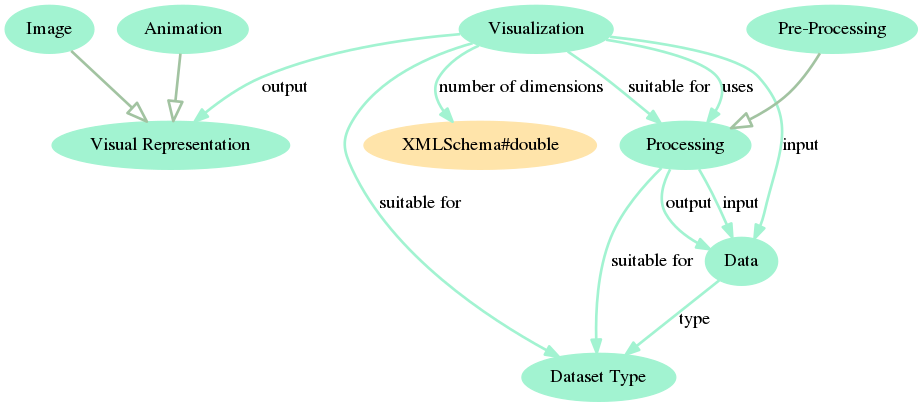
\includegraphics[height=6.7cm,width=9cm]{../figs/aavo0.01_minimum.png}
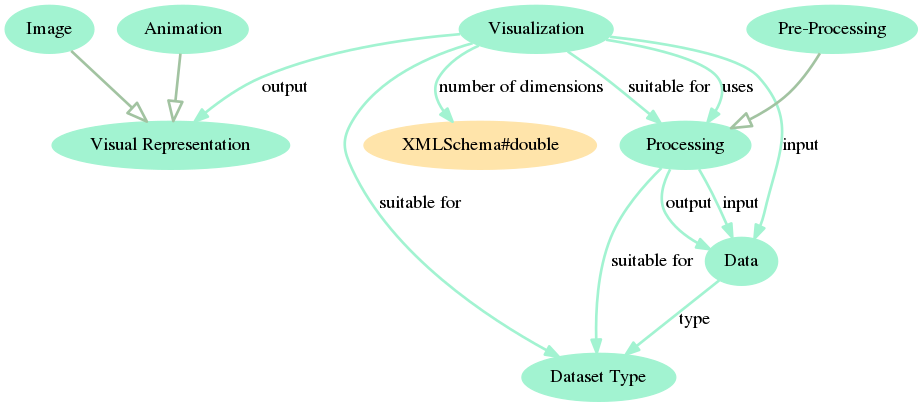
\includegraphics[width=\textwidth]{../figs/aavo0.01_minimum.png}
    \caption{}
\label{fig:minimum}%
\end{center}
\end{figure}

% potential enhancements, from the email to cristina

\subsection{AAVO example expansion}
\begin{figure}[!htbp] %h or !htbp
\vspace{-2pt}
\begin{center}
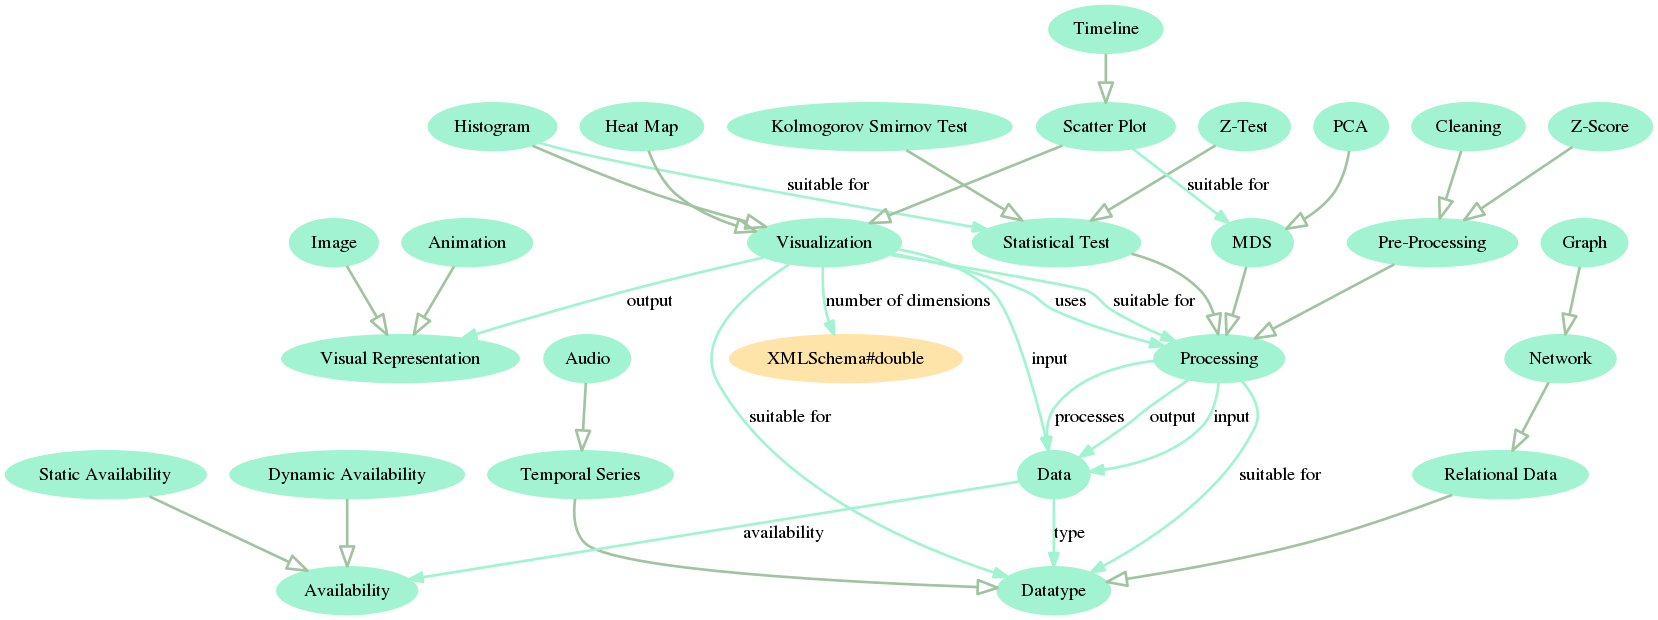
\includegraphics[width=\textwidth]{../figs/aavo0.01_exemplified.png}
    \caption{}
\label{fig:minimum}%
\end{center}
\end{figure}

\section{CONCLUSIONS AND FURTHER WORK}\label{sec:con}



\subsection*{\textit{Acknowledgements}}
The authors thank CNPq and FAPESP for the fundings received while researching the topic of this article,
the researchers of IFSC/USP and ICMC/USP for the recurrent collaboration in every situation
where we needed directions for investigation.

% ------------------------------------------------------------------------
\begin{thebibliography}{99}
\fontsize{11}{0}\selectfont
\bibitem[Bechhofer \& Miles, 2008]{owlSkos}
	Bechhofer, S., \& Miles, A. (2008). Using OWL and SKOS. Note of the SWD W3C working group.
From \url{https://www.w3.org/2006/07/SWD/SKOS/skos-and-owl/master.html}

\bibitem[Fabbri \& Oliveira, 2016]{losd}
	Fabbri, R., \& de Oliveira, O. N. (2016). Linked Open Social Database. Github repositories, from \url{https://github.com/ttm/linkedOpenSocialDatabase/raw/master/paper.pdf}

\bibitem[Fabbri, 2017]{fabbri1}
Fabbri, R. (2017). Topological stability and textual differentiation in human interaction networks:
		statistical analysis, visualization and linked data. Doctoral thesis.
		From \url{https://github.com/ttm/thesis/raw/master/thesis-rfabbri.pdf}

\bibitem[Fabbri, 2014]{pnud5}
Fabbri, R. (2014). Social participation ontologies and rules to fuel a social participation linked data cloud.
	Technical report for the United Nations Development Program.
		From \url{https://github.com/ttm/pnud5/raw/master/latex/produto.pdf}

\bibitem[Fabbri et al., 2015]{ops}
Fabbri, R., de Luna, R. B., Martins, R. A. P., Amanqui, F. K. M., \& Moreira, D. D. A. (2015). Social Participation Ontology: community documentation, enhancements and use examples. arXiv preprint arXiv:1501.02662.

\bibitem[Hitzler \& Janowicz, 2013]{semApr}
Hitzler, P., \& Janowicz, K. (2013). Linked Data, Big Data, and the 4th Paradigm. Semantic Web, 4(3), 233-235.

\end{thebibliography}
% ------------------------------------------------------------------------

%For papers written in Portuguese or Spanish.

%\begin{center}
%  TITLE IN ENGLISH
%\end{center}

%\def\abstractname{Abstract}%

%\begin{abstract}
%   Abstract in english
%\end{abstract}

%\keywords{\em{Keywords in english}}

\end{document}
